\section{Cr�er un exercice}
\subsection{Page principale}
Nous allons d�tailler dans cette partie le sc�nario de cr�ation d'un exercice.
L'enseignant cr�er un exercice en cliquant sur le lien "Cr�er un exercice" dans la zone de lien.
Il existe deux mani�res de cr�er un exercice:
\begin{itemize}
\item Soit il reprend un exercice qui existe dans la base : lien {\it � partir d'un exercice existant dans la base}
\item Soit il en cr�e un nouveau : lien {\it un nouvel exercice}
\end{itemize}
	
\begin{flushleft}
\scalebox{0.5}{\includegraphics{../eps/exercice.eps}}\\
{\it Page principale}
\end{flushleft}

\subsection{A partir d'un ancien}
\begin{flushleft}
\scalebox{0.5}{\includegraphics{../eps/exerciceList.eps}}\\
{\it L'enseignant doit s�lectionner un exercice dans la base.
Il s�lectionne l'exercice dans le navigateur.}
\end{flushleft}

\subsection{Nouvel exercice}
Il existe deux mani�res de cr�er un nouvel exercice:
\begin{itemize}
\item Soit l'enseignant importe un fichier XML depuis son compte.
\item Soit il �dite directement l'exercice dans l'�diteur de bord.
\end{itemize}
\begin{flushleft}
\scalebox{0.5}{\includegraphics{../eps/exerciceNouveau.eps}}\\
{\it Cr�ation d'un nouvel exercice}
\end{flushleft}

\subsection{Import}
\begin{flushleft}
\scalebox{0.5}{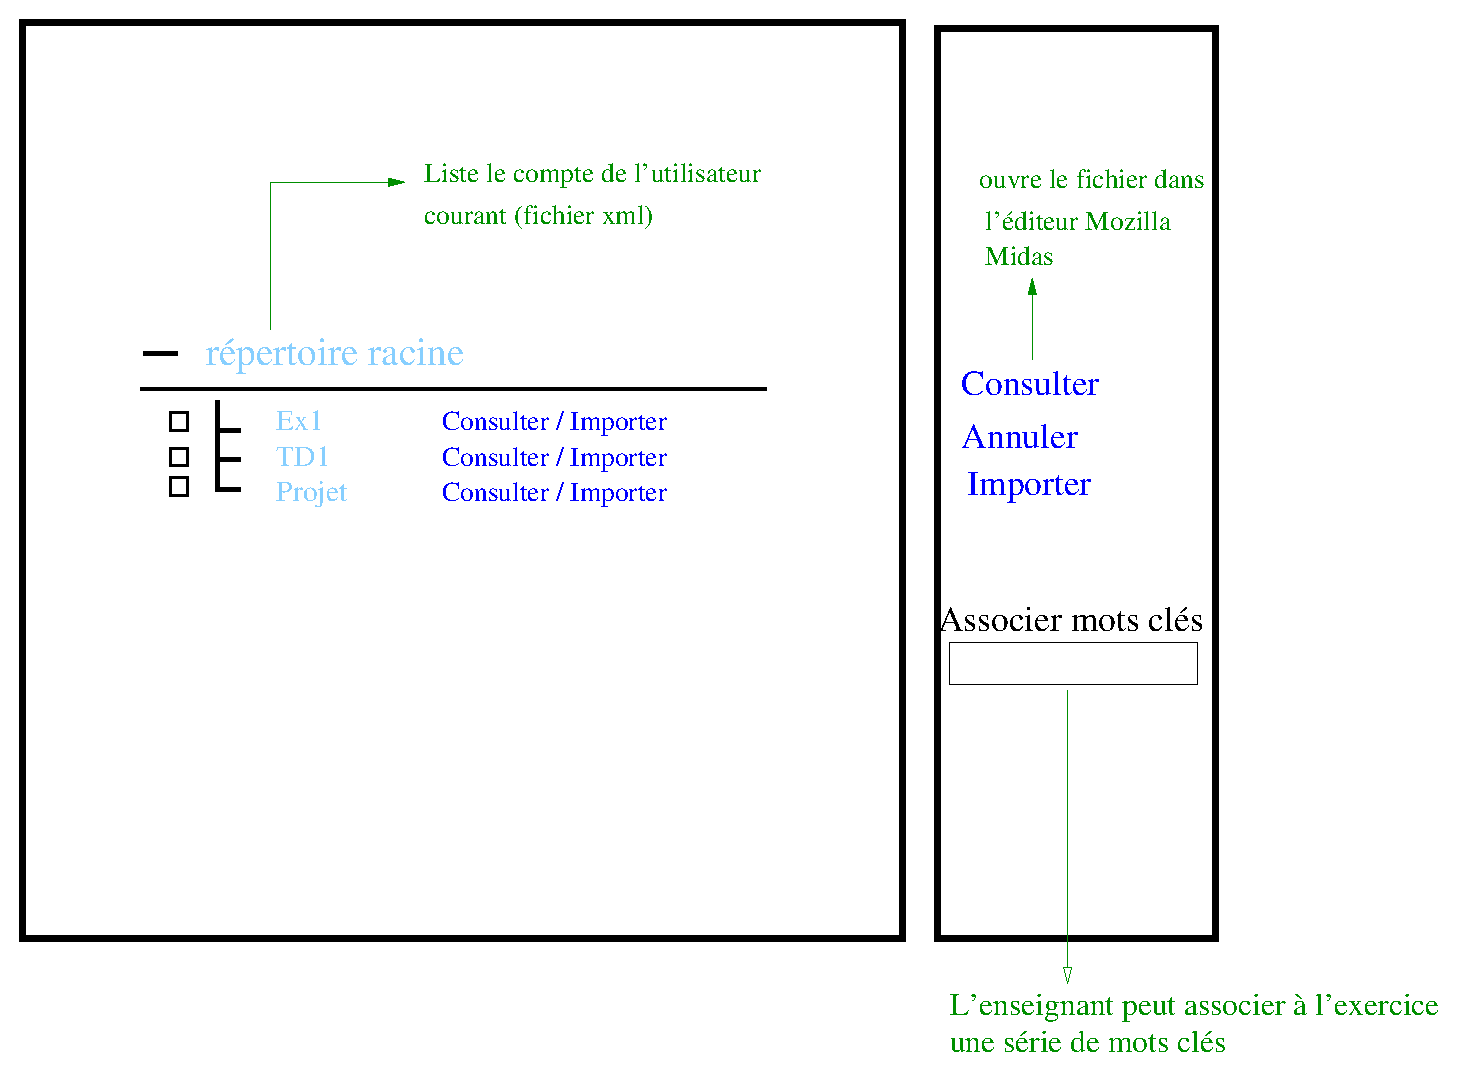
\includegraphics{../eps/exerciceExplorCompte.eps}}\\
{\it Listing du compte de l'utilisateur pour l'import}
\end{flushleft}

\subsection{Editeur de bord avec/sans balise XML}
L'�diteur de bord permet la saisie de l'exercice avec ou sans balise.

L'enseignant utilise pour la saisie de l'exercice l'�diteur embarqu�, dans la zone de visualisation.

Il existe deux mani�res d'�crire l'exercice.
\begin{flushleft}
\scalebox{0.5}{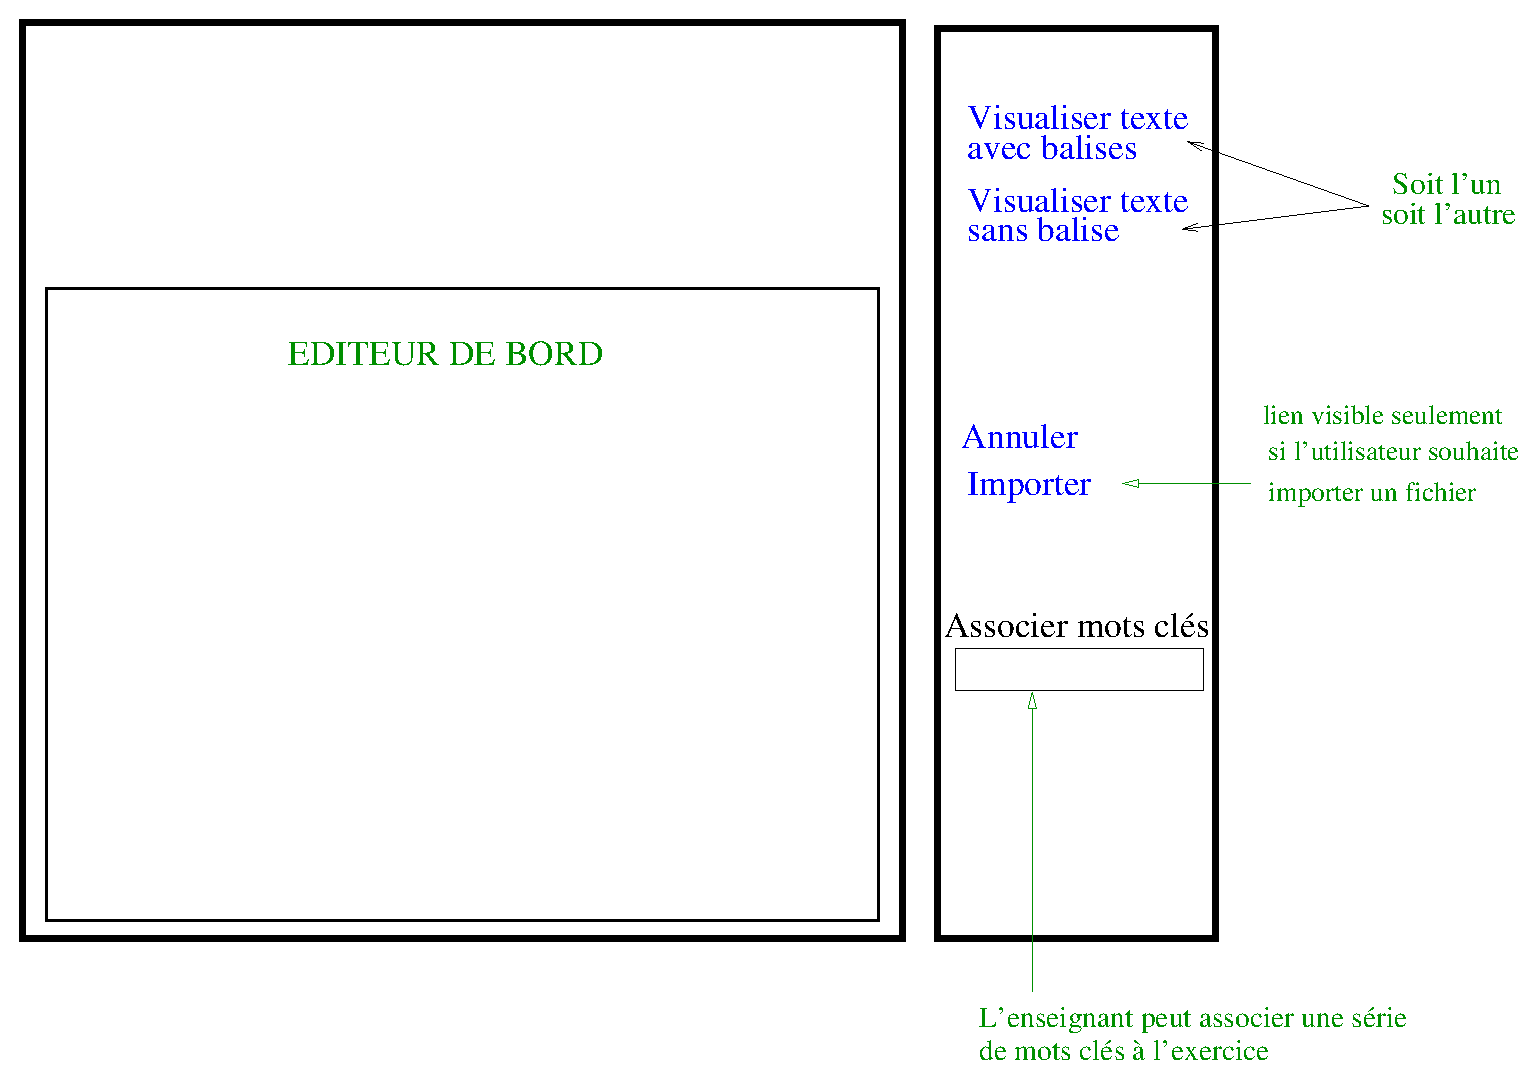
\includegraphics{../eps/exerciceEditText.eps}}\\
{\it L'enseignant saisie l'exercice directement en XML ou sans balise
selon le mode s�lectionn�}
\end{flushleft}

